\chapter{Stílusok}
\thispagestyle{empty}

Stílusok segítségével előre meghatározott formátumok
összességét alkalmazhatjuk egyetlen kattintással. Használata
megkönnyíti a munkafüzetekben és a munkalapokon egységes
stílusjegyek kialakítását. Használatához a
\textbf{Stílusok és formázás} ablakot kell megjeleníteni,
amit a \textbf{Formázás} eszköztár első kapcsolójával, a
\textbf{Formátum} menüpont megegyező nevű parancsával,
vagy az F11 funkcióbillentyűvel tehetünk meg. Az ablak első
két ikonjával a stílusok két kategóriája között
választhatunk. Ezek a Cellastílusok és Oldalstílusok. A
cellastílusok cellákra és cellatartományokra alkalmazhatók, az
oldalstílusok pedig a munkafüzet nyomtatási beállításait
tartalmazzák. Mindkét kategória alapértelmezett stílusokat
tartalmaz, ezeket módosíthatjuk, de létrehozhatunk általunk
meghatározottakat is.


\section{Stílusok alkalmazása és módosítása}

Cellastílust a formázni kívánt cella, cellák vagy
cellatartományok kijelölése után a stílus nevén kettős
kattintással állíthatunk be. Oldalstílus alkalmazásához
kattintsunk duplán a stílusra.

Cellastílust egyszerűen alkalmazhatunk több cellára és
cellatartományra a \textbf{Kitöltés formátummal}  parancs
alkalmazásával (\ref{StílusokFormázás} ábra). Egy stílust kiválasztva
húzással alkalmazhatjuk azt a kívánt elemekre. Az egér
mutatója ilyenkor a parancs ikonjához hasonló formát vesz fel a
munkalap celláin. A \textbf{Kitöltés formátummal}
kikapcsolásához kattintsunk ismét az ikonjára.

\begin{figure}[!h]
\begin{center}
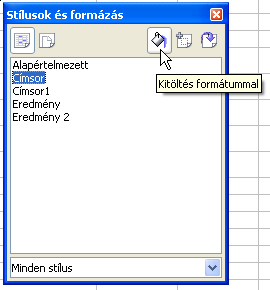
\includegraphics[width=6.644cm]{oocalcv2-img157.png}
\caption{Stílusok és formázás}\label{StílusokFormázás}
\end{center}
\end{figure}

Egy stílus módosításához a jobb egérgombbal kattintsunk a
módosítandó stílus nevén, és a megjelenő
gyorsmenüből a \textbf{Módosítás} parancsot válasszuk
(\ref{StílusMódosítása} ábra).

\begin{figure}[!h]
\begin{center}
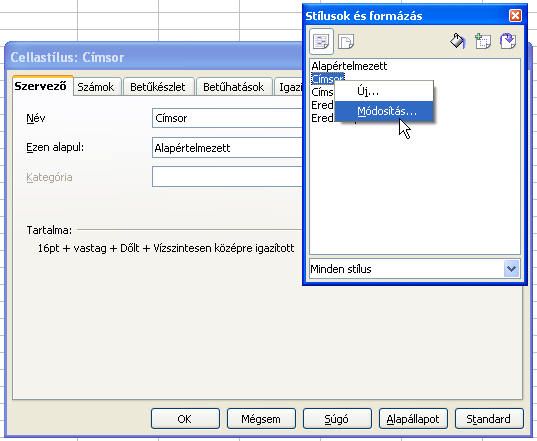
\includegraphics[width=14.208cm]{oocalcv2-img158.png}
\caption{Stílus módosítása}\label{StílusMódosítása}
\end{center}
\end{figure}

A \textbf{Cellastílus} ablak megegyezik a \textbf{Cellák
formázása} ablakkal kibővítve egy első Szervező
nevű füllel. Itt látjuk a stílus nevét, annak a stílusnak
a nevét amelyik alapjául szolgál és a formátumok
felsorolását amelyeket beállít.

A stílusok alkalmazásával formázott munkafüzetet
egyszerűen és gyorsan módosíthatunk, hiszen a stílus
formátumának módosítása minden olyan cella formátumát
módosítja, amit ezzel a stílussal előzőleg formáztunk.


\section{Stílusok létrehozása}

Az alapértelmezett stílusok módosítása helyett
létrehozhatunk saját stílusokat. Ezt legegyszerűbben egy
megformázott cella alapján a \textbf{Cellák formázása} ablak
negyedik, \textbf{Új stílus a kijelölés alapján} paranccsal
tehetjük meg. A megjelenő ablakban meg kell adni az új stílus
nevét. A stílus az előzőleg megformázott aktív cella
minden formátumát tartalmazza.

Új stílust létrehozhatunk gyorsmenü segítségével is, egy
stílus nevén jobb egérgombbal kattintva. Itt az \textbf{Új}
parancsot kell választani és megadni a stílus nevét.


\section{Feltételes formázás}

Feltételes formázás segítségével megoldható, hogy
cellánként akár három feltételt is megadjunk, amelyeknek
teljesülniük kell ahhoz, hogy a kijelölt cellák egy adott
formátumot kapjanak. A formátumokat stílusok megadásával
határozhatjuk meg. A \textbf{Formátum} eszköztár
\textbf{Feltételes formázás} párbeszédablakban
állíthatjuk be a feltételeket és adhatjuk meg a stílust. 
\Aref{FeltételesFormázás} ábrán azt a beállítást látjuk ami az aktív cellán
az Eredmény nevű stílust állítja be, ha a cella tartalma 4
és 6 között van.

\begin{figure}[!h]
\begin{center}
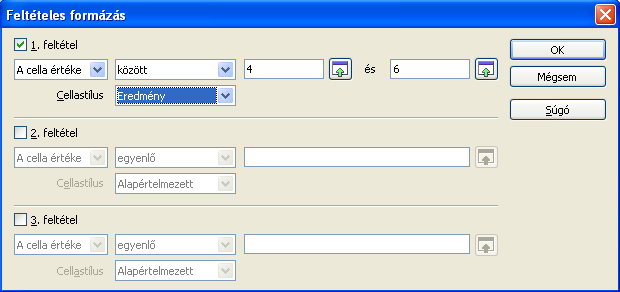
\includegraphics[width=15.999cm]{oocalcv2-img159.png}
\caption{Feltételes formázás}\label{FeltételesFormázás}
\end{center}
\end{figure}

Formázási feltételként képletet is megadhatunk. Ehhez
válasszuk \textbf{A cella értéke} helyett \textbf{A képlet
}elemet, majd adjuk meg a képletet, melynek logikai IGAZ eredménye
esetén a kiválasztott cellastílust alkalmazza a program. A
képletben használhatunk abszolút, vegyes és relatív
cellahivatkozást is, cella másolásánál az általános
szabályok szerint módosítja ezeket a Calc.

Egy cellán beállított feltételes formázást a
\textbf{Formátumecset} vagy az \textbf{Irányított beillesztés}
segítségével vihetjük át egy másik cellára, vagy
tartományra.


\section{Irányított beillesztés}

A Calcban egy lemásolt cella tartalmát nem csak a hagyományos
módon illeszthetjük be. Az \textbf{Irányított beillesztés}
használatakor megjelenő párbeszédablakban beállíthatjuk,
hogy a másolt cella milyen tulajdonságait illesztjük be.
Különböző műveleteket is végezhetünk a
beillesztésre kerülő adatokkal.

A \textbf{Mindent beilleszt} kapcsoló alapértelmezés szerint
aktív, ekkor a cella tartalma és formátumai is beillesztésre
kerülnek. Ezt kikapcsolva bejelölhetünk különböző
tulajdonságokat, és csak azok kerülnek beillesztésre. Az
Irányított beillesztés párbeszédablakot a
\textbf{Szerkesztés} menüből tudjuk előhívni, de ehhez
használhatjuk a gyorsmenüt is.

Következő lépésként vizsgáljuk meg az irányított beillesztés alkalmazását.
Amennyiben szükségünk van egy véletlen, 0 és 100 közötti
számokból álló számoszlopra, azt létrehozhatjuk az első
cellába a \textbf{=CSONK(100*VÉL())} kifejezést
írva és lefelé másolva (\ref{IrányítottBeillesztés} ábra).
Ez a számoszlop minden
cellaműveletkor újragenerálódik, az értékei
megváltoznak. Az N2:N13 tartományt kijelölve, azt menüből 
vagy billentyűkombinációval másolva, és az
irányított beillesztés ablakban a \textbf{Számok}
rádiógombot bekapcsolva az O2:O13 tartományba csak a
számértékek kerülnek át. Az eredeti N2:N13 tartományt
törölhetjük.

\begin{figure}[!h]
\begin{center}
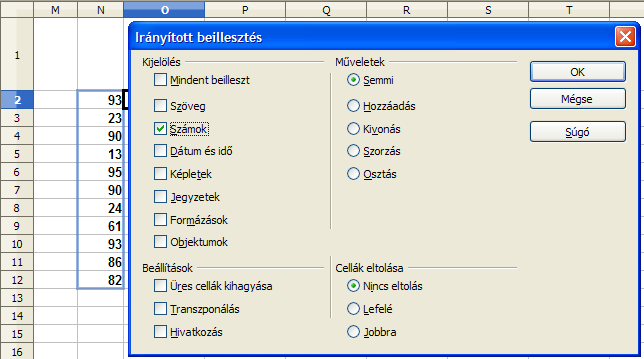
\includegraphics[width=15.999cm]{oocalcv2-img160.png}
\caption{Irányított beillesztés}\label{IrányítottBeillesztés}
\end{center}
\end{figure}


\section{Tartalom törlése}

A \textbf{Delete} billentyű lenyomásakor vagy a
\textbf{Szerkesztés} menü \textbf{Tartalom törlése} parancsra
megjelenő ablakban az irányított beillesztéshez hasonló
feltételek közül választhatunk, meghatározva az aktív cella
vagy kijelölt tartomány törlendő tartalmát, vagy
formátumát (\ref{TartalomTörlése} ábra).

\begin{figure}[!h]
\begin{center}
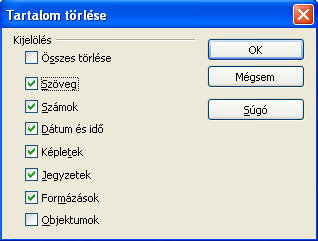
\includegraphics[width=8.414cm]{oocalcv2-img161.png}
\caption{Tartalom törlése}\label{TartalomTörlése}
\end{center}
\end{figure}


\section{34. feladat}

{\itshape
A 12. feladat táblázatában oldjuk meg feltételes formázás
és irányított beillesztés használatával, hogy a 3 alatti
átlaggal rendelkező tanulók nevei félkövér, dőlt
formátummal és szürke háttérszínnel jelenjenek meg.}

Első lépésként hozzunk létre egy stílust
,,lemarad'' néven a feladatban
megadott formátumokkal. Az első tanuló nevének celláján
válasszuk a feltételes formázást. Itt válasszuk \textbf{A
képlet} elemet. A képlet mezőt választva kattintsunk az I2
cellára. A cellacím abszolút hivatkozásként jelenik meg, ezt
változtassuk relatívra és írjuk be a feltételt
(\ref{34-feladatFeltételes} ábra).

\begin{figure}[!h]
\begin{center}
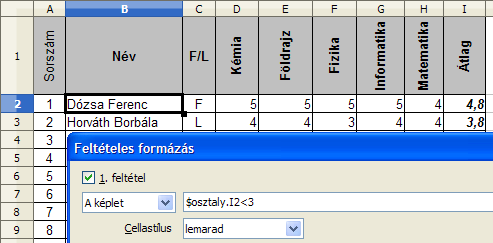
\includegraphics[width=13.042cm]{oocalcv2-img162.png}
\caption{34. feladat --  feltételes formázás}\label{34-feladatFeltételes}
\end{center}
\end{figure}

Beállítva a feltételes formázást a cella formátuma nem
változik, hiszen az első tanuló átlaga nagyobb mint 3.
Másoljuk a B2 cellát és jelöljük ki a többi tanuló
nevét, vagyis a B3:B10 tartományt. Irányított beillesztés
segítségével csak a \textbf{Formázások}at illesszük be. A
feltételes formázás minden cellán olyan beállításokkal
jön létre, hogy a tanulók nevei a saját átlaguk alapján
kapnak formátumot (\ref{34-feladatMegoldás} ábra).

\begin{figure}[!h]
\begin{center}
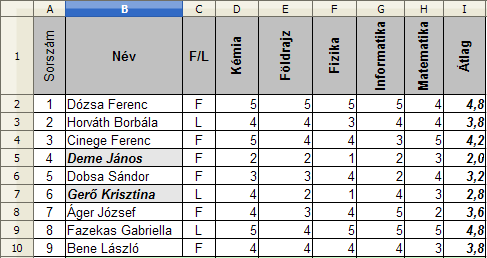
\includegraphics[width=12.883cm]{oocalcv2-img163.png}
\caption{34. feladat --  megoldás}\label{34-feladatMegoldás}
\end{center}
\end{figure}

